\documentclass[aip, rsi, amsmath, amssymb, reprint, author-year, longbibliography]{revtex4-1}

\usepackage{graphicx}% Include figure files
\usepackage{dcolumn}% Align table columns on decimal point
\usepackage{bm}% bold math
\usepackage{lipsum}
\usepackage{listings}
\usepackage{pgfplots}
\usepackage[%
  colorlinks=true,
  urlcolor=blue,
  linkcolor=blue,
  citecolor=blue
]{hyperref}
%\usepackage[mathlines]{lineno}% Enable numbering of text and display math
%\linenumbers\relax % Commence numbering lines

\definecolor{dkgreen}{rgb}{0,0.6,0}

\lstset{frame=tb,
  language=Python,
  aboveskip=3mm,
  showstringspaces=false,
  columns=flexible,
  numbers=left,
  numbersep=3pt,
  numberstyle=\color{gray},
  basicstyle={\small\ttfamily},
  keywordstyle=\color{blue},
  commentstyle=\color{dkgreen},
  stringstyle=\color{mauve},
  breaklines=true,
  breakatwhitespace=true,
  tabsize=4,
  belowskip=-0.2cm
}

\begin{document}

\preprint{AIP/123-QED}

\title[InspectorLestrade: Predicting Eye Gaze]{InspectorLestrade: An 8-Week
  Foray into Predicting Eye Gaze}

\author{R. Christian Di Lorenzo}
 \email{rdilorenzo@regis.edu}
 \affiliation{Data Science Graduate Student, Regis University}

\date{\today}% It is always \today, today,
             %  but any date may be explicitly specified

\begin{abstract}
\end{abstract}

\keywords{deep learning, eye tracking, face alignment}
\maketitle

\section{\label{sec:level1}Introduction}

Most applications of eye tracking firmly lie within medicine or user-based
research and are dominated by specialized devices with external sensors and
wearables. With the advent of computationally feasible Deep Learning, what was
previously outside the reach of the everyday user may well be possible now.

For example, a common measure of eye strength involves saccade latency and
accuracy, that is, the ability to jump from one visual focus to another.
Currently, both the exercises and testing must be done with specialized
equipment. If the predictive power of neural networks were applied to this
problem, patients would be able to perform exercises on their own and thereby
have the tools to measure and perhaps even overcome eye disabilities.

In this work, I present my modeling process to predict from a front-facing iOS
camera the gaze location of person's eyes relative to the device's lens. Using
the data set GazeCapture from \cite{7780608} containing almost 2.5M frames, I
trained a deep convolutional neural network called
InspectorLestrade\footnote{The name ``Inspector Lestrade'' comes from the
  Sherlock Holmes series and is employed in this case because the inspector was
  always confident but not always correct. This describes the result of my
  project here due to time constraints and having hardly any previous
  experience with building neural networks.} to predict a gaze coordinate
relative to the lens as well as the probability that both eyes are within the
frame.

% Fig.~\ref{fig:epsart}%
\begin{figure}
\includegraphics[height=5.5cm]{faces-blurred-grayscale-2.png}
\caption{\label{fig:faces} A sample of the +1400 participants with bounding
  boxes of eyes and faces determined by the built-in, real-time detection system
  of iOS.}
\end{figure}

\subsection{\label{sec:level2}Background}

As a part of my Deep Learning class for my masters in Data Science, I have been
privileged to not only self-determine a project but also have the entire 8-week
semester to produce a decent model. With some knowledge of machine learning but
essentially no experience with Deep Learning, the current results of this
project are very much a work in progress and further effort would be needed
before its utility could be realized in any real situation. The detailed
limitations will be discussed further in a later section.

Due to previous interest in eye tracking from my work at a software consultancy,
I did a bit of searching and stumbled upon the work of \cite{7780608}. This data
set, named GazeCapture\footnote{Available by permission from
  \url{http://gazecapture.csail.mit.edu}}, contains data of nearly 2.5 million
images of over 1400 participants gathered via crowdsourcing. Because my goal was
to understand Deep Learning over the course of this project, I only did a
preliminary read of their paper and entirely skipped the section on their model
iTracker in order to keep my bias free.\footnote{Interestingly, several of my
  data visualizations ended up coinciding with their diagrams but were not
  actually based off of them.}

Throughout the entire process, I wrote weekly updates either directly on the
status of the project or individual bits of learning. The writings, pretrained
models, and all code are available from the repository:
\url{https://github.com/rcdilorenzo/inspector-lestrade}.

\section{\label{sec:level1}Exploratory Data Analysis}

Before considering model architectures, an exploratory data
analysis\footnote{All data visualization figures are available from the notebook
  in the repository: eye-tracking-eda.ipynb (\url{https://git.io/fxoDe})} (EDA)
revealed some important details about GazeCapture. As seen in
Fig.~\ref{fig:recordsbytype}, a variety of devices were employed through the
crowdsourced outlet which produces a good range of screen sizes from the iPhone
4S to the 12.9'' iPad Pro. Likewise, Table \ref{tab:dots} shows the maximum
extents of the data which will later be important if the model is specialized to
iOS devices.

\begin{figure}
  \includegraphics[height=5cm]{records-by-device-type.png}
\caption{\label{fig:recordsbytype} Frequency of frames taken by iOS device type.}
\end{figure}

\begin{table}[h]
\begin{ruledtabular}
\begin{tabular}{lllll}
     & XPts         & YPts         & XCam         & YCam \\ \hline
mean & 294.22       & 260.50       & 0.12         & -1.85        \\
min  & 40.00        & 40.00        & -26.52       & -26.52       \\
max  & 1326.00      & 1326.00      & 26.52        & 26.52        \\
\end{tabular}
\end{ruledtabular}
\caption{\label{tab:dots}Extent of dot information. ``Pts'' represent screen
  pixels while ``Cam'' represents centimeters from camera lens (normalized by
  the lens location on each device type).}
\end{table}

Beyond these basic numbers, a scaled representation as seen in
Fig.~\ref{fig:relativedots} illustrates the distribution of dots that
participants are asked to gaze at while their picture is repeatedly taken from
the front-facing camera. This visualization clearly indicates that all of the
primary sectors of the device were covered in addition to some uniformly random
points across the entire screen.

\begin{figure}[h]
  \includegraphics[height=7cm]{dot-values-relative.png}
  \caption{\label{fig:relativedots} Frequency and distribution of generated dots
    for each device.}
\end{figure}

For the purposes of this project, however, the most important distribution is
the absolute position of the dots in centimeters from the camera lens.
Fig.~\ref{fig:campoints} clearly shows not only the outline of multiple device
sizes--5.7'', 9.7'', and 12.9''--but also the various device
orientations--portrait, upside-down portrait, landscape left, and landscape
right. Note how the iPhone is never used in the upside-down orientation
as well as the left offset of the camera seen in the mismatched landscape iPhone
frequencies.

\begin{figure}
  \includegraphics[height=6.5cm]{cam-points-absolute.png}
\caption{\label{fig:campoints} Frequency and distribution of dots in centimeters
from the camera.}
\end{figure}

\section{\label{sec:level1}Data Preprocessing}

Both before and during the modeling stage, data preprocessing was an essential
component. To explore these details, the initial two approaches must be briefly outlined.

\subsection{\label{sec:level2} Approach 1: Object Detection of Eyes}

Although this approach was eventually dropped due to time constraints, it was
certainly sound in concept. Although \cite{7780608} included the real-time iOS
predictions of eyes and faces, my initial exploration revealed that these
bounding boxes were seriously wanting. Finding the freely available
sample\footnote{\url{https://www.figure-eight.com/dataset/open-images-annotated-with-bounding-boxes/}}
of Open Images v4 by \cite{openimages}, I employed YOLOv3 by \cite{yolov3} to
more accurately find bounding boxes labeled ``Human eye'' from Open Images.

To accomplish this task, however, the entire sample needed to be downloaded
($\sim$560 GB) in order to have all available images. From multiple
metadata files, image paths had to be cross-referenced with bounding boxes after
being filtered by tag name (i.e. ``Human eye'').

Most of the data
preprocessing\footnote{openimage-eye-detection-yolo-v3.ipynb: \url{https://git.io/fxoMp}}
consisted of transforming the Open Image metadata into the text file format
readily accepted by YOLOv3 \citep{yolov3}. For example, each bounding box was
listed as a separate row even though it referenced the same image. These had to
be grouped and then assigned a numerical class identifier (in this case just 0
for a single class). Below is a sample of the produced text file.

\begin{lstlisting}
openimagesv4/train_08/000004f4400f6ec5.jpg 489,509,274,303,0 618,645,216,232,0 675,696,219,229,0
openimagesv4/train_08/0000271195f2c007.jpg 424,522,429,486,0 573,650,440,494,0
...
\end{lstlisting}

\subsection{\label{sec:level2} Approach 2: Face Landmarks}

The second approach begins with an external deep neural network that identifies
facial landmark features in 3D-space. Using the face-alignment network of
\cite{bulat2017far}, points of the jaw, mouth, nose, eyebrows, and eyes are
projected into 3D space even when certain portions of the face do not entirely
appear in the frame.

\begin{figure}[b]
  \includegraphics[height=9cm]{landmarks-to-eyes.png}
  \caption{\label{fig:landmarktransform} Transforming landmarks to 128x128 eye
    images.\footnote{\label{ftn:preprocessing}face-landmarks-modeling-preprocessing.ipynb:
      \url{https://git.io/fxoSN}}}
\end{figure}

From these facial features, a bit of data preprocessing was performed to produce
the necessary inputs for InspectorLestrade--128x128 images of the left and right
eyes as well as the scaled landmark points (Fig.~\ref{fig:landmarktransform}).
Several hurdles had to be overcome to produce a successful slice for every set
of facial landmarks.\footnote{facial-model.py: \url{https://git.io/fxoS9}} For
example, sometimes the landmarks fall outside of the image such as when only
half of a face is visible. Because InspectorLestrade always expects the same
size inputs, it was necessary to create a 1px vertical slice closest to the
``invisible'' eye and then expand it to the expected 128x128 size. As will be
seen later, this became a hurdle for the modeling process.

For the training process, these eye images needed be sliced either on the fly or
beforehand. Due to the longer computational complexity of predicting these
landmarks over slicing the images, I opted to run the face-alignment network
across all the frames in preparation for training InspectorLestrade. Although
the preprocessing of the landmarks took nearly an entire week to save the
results in batches,\footnote{landmark-generator.py: \url{https://git.io/fxoSG}} it
enabled slicing images on the fly and thereby more concentrated focus on
modeling InspectorLestrade.

Additionally, the raw points from the face-alignment library
\citep{bulat2017far} needed to be scaled. Using the distribution of the $x$, $y$,
and $z$ values, `StandardScaler' from `sklearn' could be used to create smaller
values for better neural network performance.$^\text{\ref{ftn:preprocessing}}$
This distribution information is then saved for later retrieval during prediction.

\begin{figure}[b]
  \includegraphics[height=7cm]{inspector-lestrade-overview.jpg}
  \caption{\label{fig:overview} Visual overview of the inputs and outputs of InspectorLestrade.}
\end{figure}

All of these preprocessing elements are brought together into the
`InspectorLestradeGenerator'\footnote{generator.py: \url{https://git.io/fxoHF}}
that takes the original GazeCapture data frame plus the pre-generated landmarks.
In turn, it renders the inputs and outputs for training. The inputs include the
three elements seen in Fig.~\ref{fig:overview} while the outputs include an $(x,
y)$ coordinate as well as a boolean output of whether both eyes were visible
(roughly corresponding to whether the person is actually looking at the screen
at all).

\section{\label{sec:level1}Modeling}

\subsection{\label{sec:level2} Approach 1: Object Detection of Eyes}

With Python and keras chosen as the primary technologies for the class, I
employed a keras version\footnote{\url{https://github.com/qqwweee/keras-yolo3}}
of the YOLOv3 architecture that provided a decent example of
retraining the existing weights for a new object classification problem. In a
transfer learning problem such as this first approach, freezing most of the
layers for the first phase of training is common. As seen in
Fig.~\ref{fig:yoloinitial}, I experimented with the learning rate, number of
frozen layers, and number of images.\footnote{All of these tweaked models are
  based off of the YOLOv3-320 weights trained on the COCO data set. See
  \url{https://pjreddie.com/darknet/yolo}.}

\begin{figure}[h]
\includegraphics[height=4cm]{yolo-loss-initial.png}
\caption{\label{fig:yoloinitial} TensorBoard snapshot of first 35 steps of
  YOLOv3 training with various data sizes, learning rates, and frozen layers.}
\end{figure}

For the initial phase, it proved that the fourth version (named
``v4-12k-adam1e3-train10'') proved to be the most successful of the various
iterations as it was more stable even than the second full version. Decoding the
name of this version, v4 included 12000 images, a learning rate of 0.001, and 10
layers of unfrozen layers (i.e. layers whose weights and biases were updated).
Continuing the long training process for v4, the final validation loss ended at
7.847 after almost 24 hours of training on a 1080 Ti (Fig.~\ref{fig:yoloval}).
Although bounding box detection of eyes does not actually predict coordinates,
this approached was dropped due to the better performance of the second approach
at the time and due to time constraints.

\begin{figure}[t]
\includegraphics[height=4cm]{yolo-final-val-loss.png}
\caption{\label{fig:yoloval} Final steps of the v4 model after unfreezing all of
  the layers and allowing the Adam optimizer to shrink the learning rate.}
\end{figure}

\subsection{\label{sec:level2} Approach 2: Face Landmarks}

As previously described, the primary model InspectorLestrade needs to predict
coordinates based on the landmarks from the face-alignment library as well as
the left and right eye images. Although I produced twelve separate architectures
over the course of 3 weeks, the sixth iteration ended up with the best results.
Through many failures, a little bit of success, and a lot of learning, I
produced a decent 30-layer architecture with a trained weight size of 477KB.

For the train, test, and validation data sets, the original data was filtered by
the frames that had detected facial landmarks and then split based on the
researchers' original split. As seen in Fig.~\ref{fig:tvtsplit}, the train data
set consists of nearly 1.6M frames.

\begin{figure}[h]
\includegraphics[height=4cm]{train-val-test-split.png}
\caption{\label{fig:tvtsplit} Split of train/test/validation by frames.}
\end{figure}

\subsubsection{\label{sec:level3} Basic Intuition}

In this image-based problem, perhaps the most basic intuition is that
convolutional layers with pooling operations will be required. Although current
research suggests that other techniques such as capsule layers may provide
better results, all of the top-performing image-based architectures since 2014
have employed some combination of these two layer types. This pattern of
convolutional layers should be symmetrical for the left and right eyes with
repeated blocks of Conv2D layers and MaxPooling2D keras layers.

In a regression problem and boolean problem such as this one, the chosen
activation function for each layer in the network is critical for reasonable
success. For the coordinate output, the activation function should be able to
produce a semi-unconstrained output at least within the range of $[-26.52,
26.52]$ (Table \ref{tab:dots}). For the gaze likelihood output, its function
should only produce values of $[0, 1]$ since it represents a numerically-encoded
boolean. Backtracking from these function requirements, hidden layers only
present for that particular output should be tailored to that range.

\subsubsection{\label{sec:level3} Loss Function}

With the realization of the ``invisible eye'' problem that produces an eye with
essentially ``garbage'' image data (stretched from a 1px strip), the network now
has three outputs. Whereas the mean-squared error (MSE) of simple Euclidean
distance in 2D was previously acceptable to measure accuracy, the third boolean
value complicates the loss function. While keras does allow for performing a
metric separately on different outputs, it does not seem to support using
different metrics for different outputs. If a network had two loss functions, it
would be quite difficult if not impossible to take the partial derivative with
respect to each simultaneously for the backpropagation phase. Therefore, some
combination function is needed that contains a gradient for each variable.

Conceptually, the goal is to penalize the distance by a factor that describes
the delta of predicted versus actual probability that both eyes are visible. If
the network predicts that both eyes are visible but one is actually not, the
loss should be described as the Euclidean distance times some factor larger than
1. Additionally, the Euclidean distance should be returned if the probability
output is perfectly correct. Assembling these requisites, a satisfying equation
combines a delta between 1 and 2 (the factor) and the original loss function.
\vspace{3mm}

{\small
\begin{math}
\begin{aligned}
    g_{\text{loss}} &= (\hat{g} - g)^2 + 1\; \text{(as multiplicative error factor)}\\
    \text{MSE} &= \frac{1}{b}\sum_{i=1}^b(\text{factor}\cdot\text{distance})^2\\\\
    \text{Loss} &= \frac{1}{b}\sum_{i=1}^b\left[\left((\hat{g_i} - g_i)^2 + 1\right)\cdot\sqrt{(\hat{y_i} - y_i)^2 + (\hat{x_i} - x_i)^2}\right]^2\\
    &= \frac{1}{b}\sum_{i=1}^b\left[(\hat{g_i} - g_i)^2 + 1\right]^2\left[(\hat{y_i} - y_i)^2 + (\hat{x_i} - x_i)^2\right]
\end{aligned}
\end{math}
}

\setlength\parindent{0pt}
This equation is quite easily translated into a tensorflow operation.
\setlength\parindent{10pt}

\begin{lstlisting}
def loss_func(actual, pred):
    x_diff = tf.square(pred[:, 0] - actual[:, 0])
    y_diff = tf.square(pred[:, 1] - actual[:, 1])
    g_diff = tf.square(pred[:, 2] - actual[:, 2])

    return K.mean(tf.square(g_diff + 1) *
                   (y_diff + x_diff))
\end{lstlisting}

\subsubsection{\label{sec:actfunc} Activation Functions}

Although the sixth iteration of the InspectorLestrade architecture did not
include a custom activation (but instead used linear), I did experiment quite a
bit\footnote{\url{https://rcd.ai/eye-tracking-nn-activation-functions}} with
custom activation functions especially when the loss values were in the range of
$[10^9, 10^{24}]$. Most of these functions (Fig.~\ref{fig:actplots}) are a
variation of the sigmoid function in order to allow for a finer output even when
the input to the function is more granular.

\begin{figure}
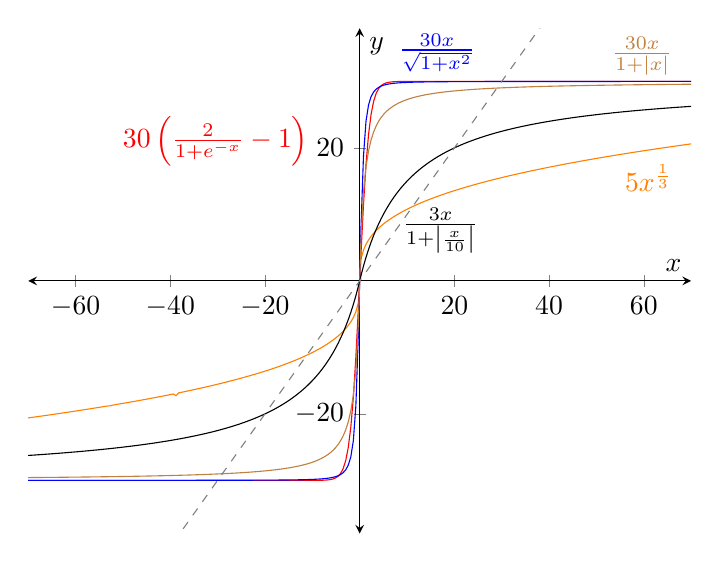
\begin{tikzpicture}[>=stealth]
    \begin{axis}[
        xmin=-70,xmax=70,
        ymin=-38,ymax=38,
        axis x line=middle,
        axis y line=middle,
        axis line style=<->,
        xlabel={$x$},
        ylabel={$y$},
        width=10cm,
        height=8cm,
        ]
        \addplot[no marks,orange,<->] expression[domain=-80:80,samples=300]{5*x/abs(x)*abs(x)^(1/3)} 
                    node[pos=0.85,anchor=north west]{$5x^{\frac{1}{3}}$};
        \addplot[no marks, red,<->] expression[domain=-80:80,samples=300]{30*(2/(1+e^(-x))-1)} 
                    node[pos=0.6,xshift=-18pt,anchor=east]{$30\left(\frac{2}{1+e^{-x}}-1\right)$};
        \addplot[no marks, blue,<->] expression[domain=-80:80,samples=300]{(30*x)/(sqrt(1+x^2))} 
                    node[pos=0.7,anchor=south]{$\frac{30x}{\sqrt{1 + x^2}}$};
        \addplot[no marks, brown,<->] expression[domain=-80:80,samples=300]{(30*x)/(1 + abs(x))} 
                    node[pos=0.9,anchor=south]{$\frac{30x}{1 + \left|x\right|}$};
        \addplot[no marks, black,<->] expression[domain=-80:80,samples=300]{(3*x)/(1 + abs(x / 10))} 
                    node[pos=0.58,anchor=north west]{$\frac{3x}{1 + \left|\frac{x}{10}\right|}$};
        \addplot[no marks, gray,dashed] expression[domain=-80:80,samples=300]{x};


    \end{axis}
\end{tikzpicture}
\caption{\label{fig:actplots} Possible activation functions that constrain the
  output of the neural network.}
\end{figure}

\subsubsection{\label{sec:architecture} Neural Network Architecture}

Putting all of these considerations into practice, the sixth model iteration
(Fig.~\ref{fig:modelv6}) employs three groups of convolutional and pooling
operations--two groups of eight 3x3 Conv2D and 3x3-stride MaxPooling2D layers as
well as a group of four 2x2 Conv2D and 2x2-stride MaxPooling2D layers. These
groups, employed for each eye, were capped off with a BatchNormalization layer
before concatenation with the landmark pathway. The landmark path consisted
of three layers before being flattened: 16 fully-connected neurons,
BatchNormalization, and another 8 fully-connected neurons. In addition to the
common pattern of Conv2D followed by MaxPooling2D, the BatchNormalization layers
added throughout the network assist in ``centering'' the values around zero to
keep the neurons from wildly flailing with large weights and biases.

\begin{figure}
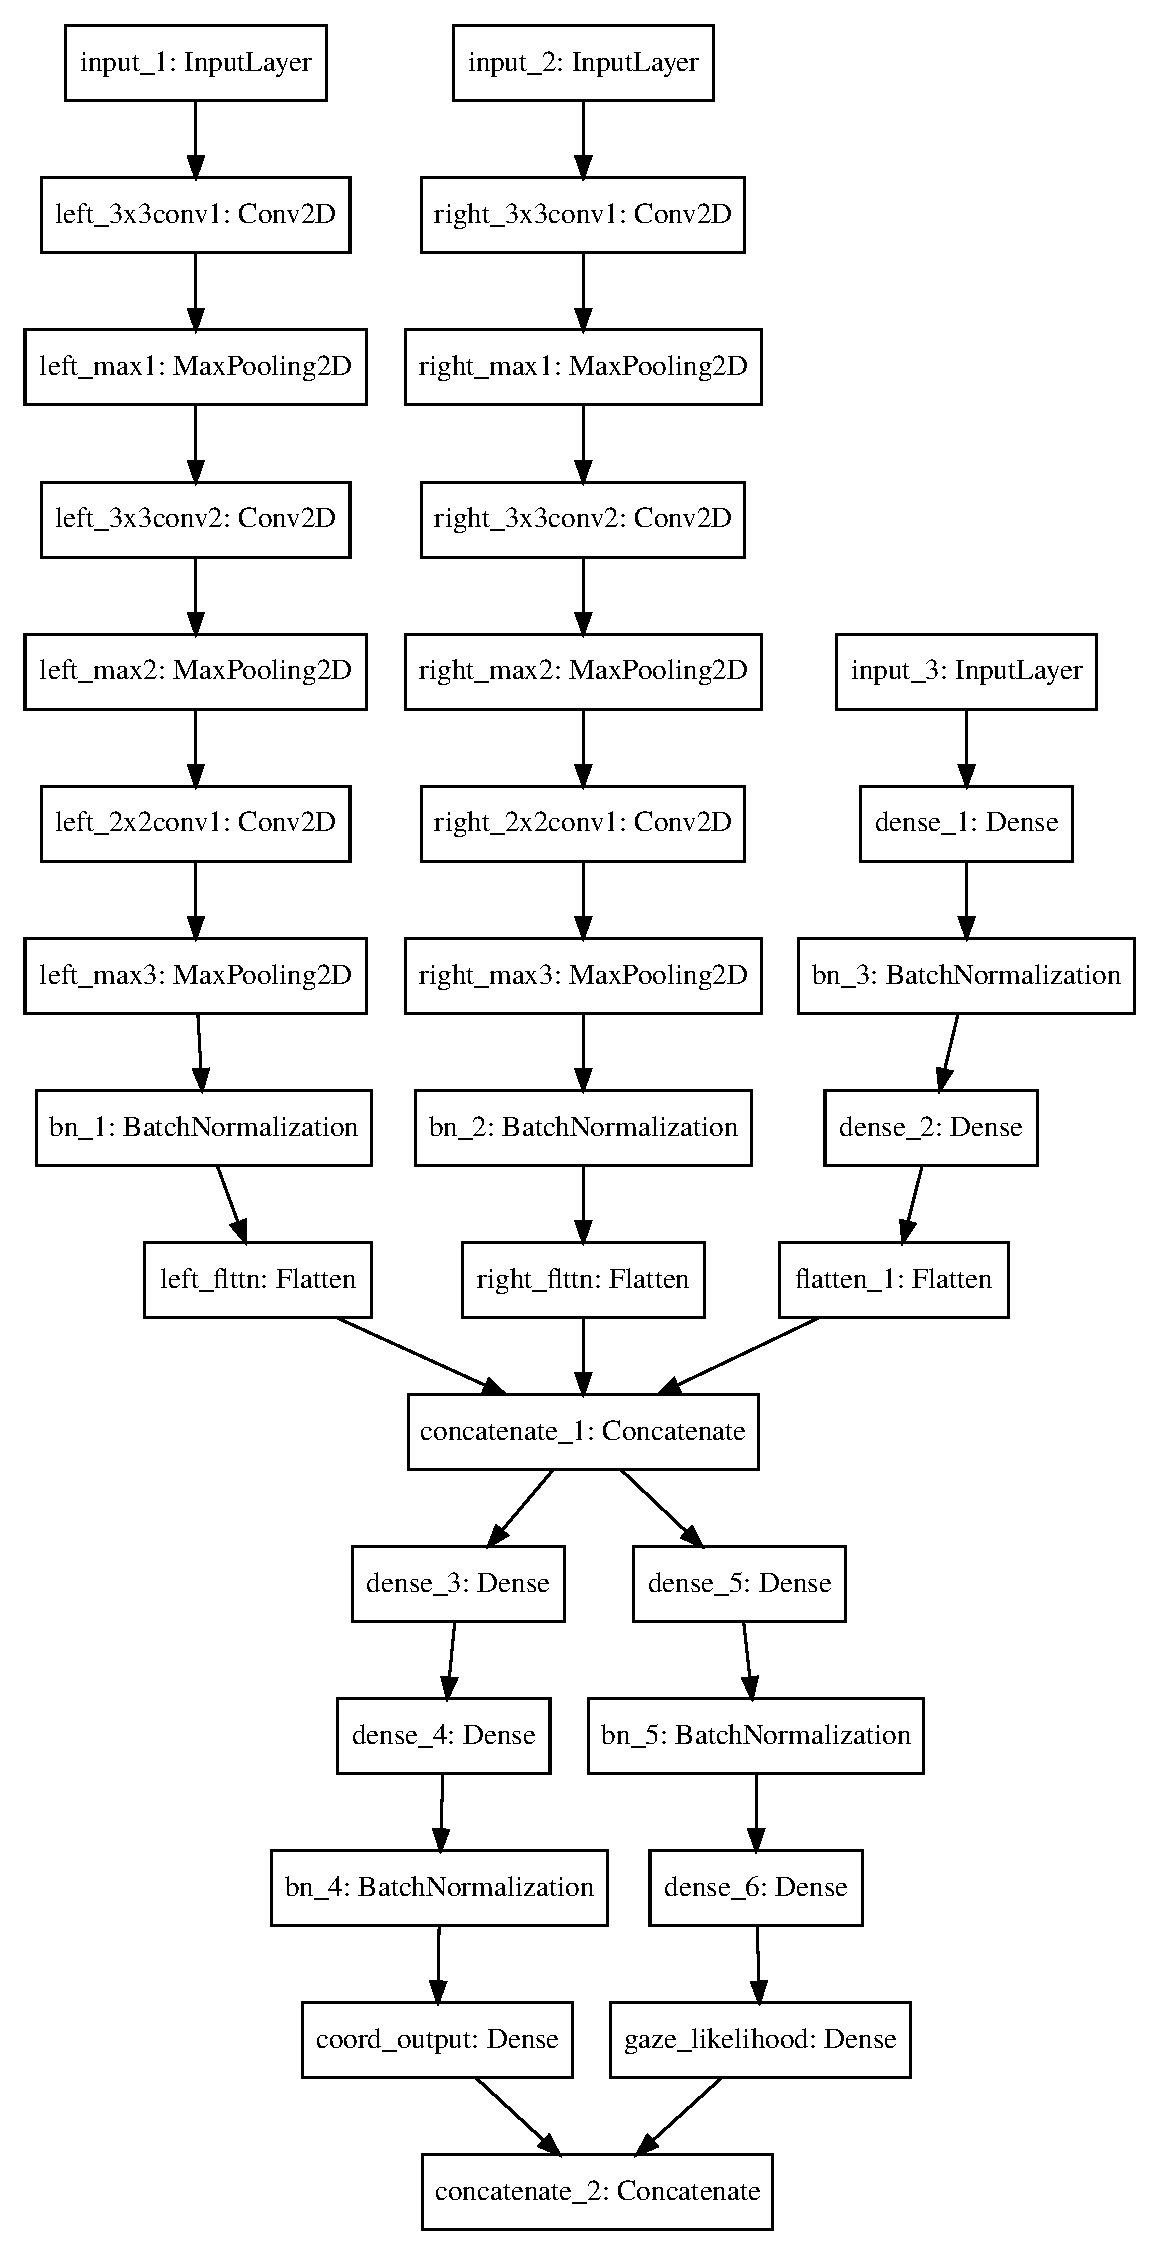
\includegraphics[height=17.5cm]{v6-lestrade.eps}
\caption{\label{fig:modelv6} InspectorLestrade architecture.\footnote{Code
    available from train.py (\url{https://git.io/fxojD})}}
\end{figure}

For the remaining two pathways leading to the coordinate and likelihood values,
a combination of diminishingly smaller Dense layers as well as
BatchNormalization are employed. The final coordinate layer uses a linear
activation function while the likelihood layer applies a sigmoid function to
represent the boolean value.

\section{\label{sec:level1}Results \& Evaluation}

\subsection{\label{sec:results} Approach 1: Object Detection of Eyes}

Although the validation set of the retrained YOLOv3-320 network achieved a loss
of 8.318, an easy test on a simple image kept indicating a significant problem
(Fig.~\ref{fig:yoloissue}). Because YOLOv3 was designed to distinguish between
multiple classes as well as perform bounding box detection, its loss function is
artificially lowered since its class prediction is always right (``Human eye'').

\begin{figure}
\includegraphics[height=4cm]{yolo-issue.png}
\caption{\label{fig:yoloissue} Sample image of retrained YOLOv3
  architecture.\footnote{eye-detection-yolo-test.ipynb:
    \url{https://git.io/fxKJm}} The extremely low class confidence ($< 0.5\%$)
  indicates a major issue.}
\end{figure}

Despite this approach being abandoned due to time constraints, I believe that it
holds promise. By reworking the data preprocessing step to include faces as a
different class, the architecture should be able to properly train. From there,
slicing the image as well as including the face and eye locations should give a
second neural network plenty of information in order to achieve a good result.
If this second network did achieve convergence, it could easily be appended as an
extension to the YOLOv3 network to output a coordinate prediction and confidence
level.

\subsection{\label{sec:level2} Approach 2: Face Landmarks}

Turning attention to the primary approach, InspectorLestrade had three
iterations that were turned out to be moderately decent. However, the original
loss function is not a good measurement of accuracy since it is not an intuitive
measurement and cannot be compared to \cite{7780608}. Instead of incorporating
likelihood as the loss function originally did, the test function collapses the
measurement to only include coordinates where both eyes of the participant were
visible and detected by the face-alignment library. The following tensorflow
operations achieve this metric.

\begin{lstlisting}
# From model.py (https://git.io/fxKTC)  

def scaled_distance_loss(actual, pred):
    combined = tf.concat([actual, pred], axis=1)
    masked = tf.boolean_mask(
        combined,
        tf.math.equal(combined[:, 2], 1.0)
    )
    x_diff = tf.square(masked[:, 0] - masked[:, 3])
    y_diff = tf.square(masked[:, 1] - masked[:, 4])
    return K.mean(tf.sqrt(x_diff + y_diff))
\end{lstlisting}

\vspace{0.5cm}
Though this mean Euclidean distance is slightly different from the original
researchers, it gives the best approximation from the network ensemble chosen.
As seen in Fig.~\ref{fig:top3models}, the sixth iteration came in at an average
of 4.35cm from the actual locations.\footnote{Detailed results and
  experimentation playground with various architectures and weights are
  available in results.ipynb (\url{https://git.io/fxKTI}).}

\begin{figure}[t]
\includegraphics[height=5cm]{lestrade-top-3-models.png}
\caption{\label{fig:top3models} Top three performing models on the test set.}
\end{figure}

Despite the test values seen in Fig.~\ref{fig:top3models}, much of the training
process had values fluctuating from $<100$ to over $10^{24}$. After many
iterations, it appears that this unusual behavior was due at least in part to
the enormous number of records per data point in TensorBoard. Each point
thereby represents only the final batch of 128 in the $\sim$1.6M frames of the
training set.

After switching just recently to a modification of the sixth iteration using 15
minute segments of only 128K images per epoch, the result of
Fig.~\ref{fig:v13taper} indicates a more traditional slope of descent.

\section{\label{sec:level1}Discussion}

\begin{figure}[t]
\includegraphics[height=3cm]{v6-bounce.png}
\caption{\label{fig:v6bounce} Bouncing loss of the sixth iteration. Note that
  the entire training set is used per epoch ($\sim$3.5 hours/epoch).}
\end{figure}

\begin{figure}[t]
\includegraphics[height=3cm]{v13-taper.png}
\caption{\label{fig:v13taper} Tapering loss of a partial thirteenth iteration.
  Note that these values only include 1000 batches per epoch.}
\end{figure}

With under eight weeks of work on this solo project having almost no prior
experience with deep neural networks, I am somewhat satisfied with the results
though a higher accuracy would have been much appreciated. That said, the
project is certainly in a position where it could quite be continued in order to
find a more accurate architecture. For example, I did not experiment much with
dropout or L1/L2 normalization layers since I was primarily focused on getting
any model to converge. Likewise, experimenting with an activation function that
forces an extreme slope at its extremes (i.e. a cubic) could be another path
forward.\footnote{This is actually the modification presented in
  Fig.~\ref{fig:v13taper} though the result is much to early to be even
  anecdotal.}

Even with the 4.35cm mean distance, though, the network needs a bit of
engineering to even be deployable. The face-alignment library
\citep{bulat2017far} uses PyTorch while InspectorLestrade employs keras. Because
they both use CUDA for GPU-acceleration but are not made to work together, it is
difficult to have them both use the GPU without hogging all of the memory for
themselves. To mitigate this problem for evaluation of new images through both
networks, I ended up setting PyTorch to use the CPU so that keras could access
the GPU.

Unfortunately, time constraints also restricted testing and tuning of the
network speed. Though I did perform some exploratory analysis of
face-alignment's speed in FPS, I was focused on accuracy with speed only as a
nice to have feature. However, the chosen YOLOv3 weights that I retrained from
actually was one of the faster models at an advertized 44 FPS \citep{yolov3}.

\begin{acknowledgments}
  This 8-week project was made possible courtesy of my Deep Learning professor,
  Geena Kim, Ph.D., from the Data Science department of Regis University. Thanks
  also to the researchers of GazeCapture and iTracker for permission to download
  and explore their data \citep{7780608}.
\end{acknowledgments}


\nocite{*}
\bibliography{references}

\end{document}